% The statement-seam claim: `statementBody` asserts that whitespace between a
% picture body's statements is insignificant to the package that consumes them,
% which is what licenses the formatter to open a new line at a seam the author
% *glued* (`…;\draw`) — the one sanctioned breach of the glued-divider
% principle, the `ContentKind::Keyval` licensing pattern. The CST oracles
% cannot see the risk (a space is trivia to the CST and content to TeX), so
% this file compiles the glued spellings and lets the before/after diff prove
% the inserted break changes nothing. The unit-glue model is exercised too:
% every statement below is long enough to force interior wraps at unit
% boundaries.
\documentclass[11pt]{article}
\usepackage[margin=2cm]{geometry}
\usepackage{tikz}
\usepackage{pgfplots}
\pgfplotsset{compat=1.18}
\begin{document}

Glued statement seams, split by the formatter onto their own lines:

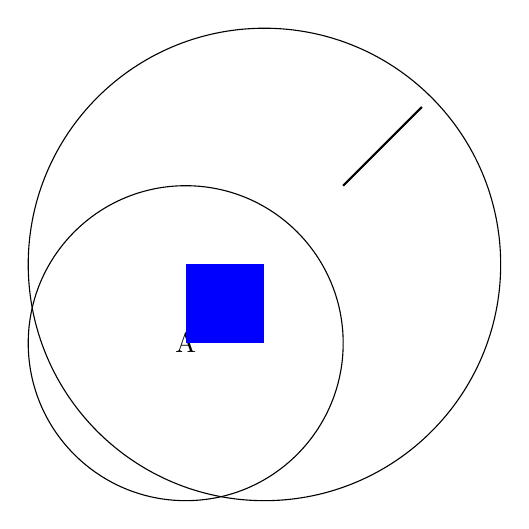
\begin{tikzpicture}
  \draw (0,0) circle (2);\draw (1,1) circle (3);\node at (0,0) {A};
  \fill[blue] (0,0) rectangle (1,1);\draw[thick] (2,2) -- (3,3);
\end{tikzpicture}

Interior wraps at unit boundaries (operator, at, coordinate/operation):

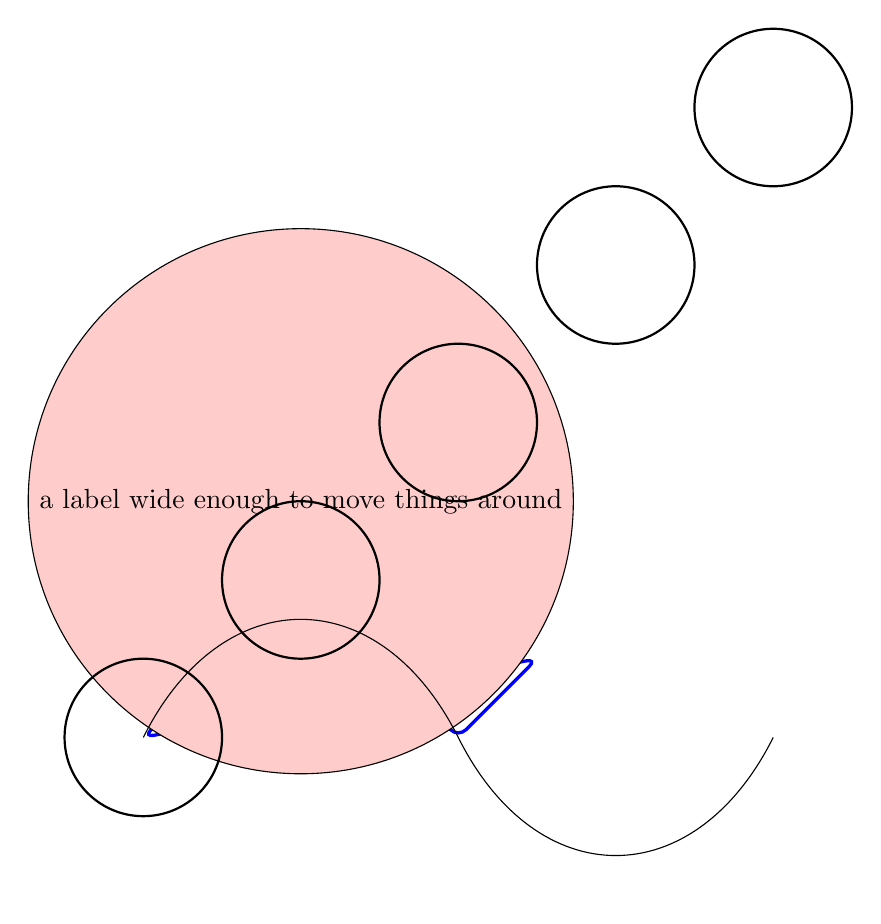
\begin{tikzpicture}
  \draw[very thick, blue, rounded corners] (0,0) -- (1,1) -- (2,0) -- (3,1) -- (4,0) -- (5,1) -- cycle;
  \node[fill=red!20, circle, draw, inner sep=4pt] at (2,3) {a label wide enough to move things around};
  \draw[thick] (0,0) circle (1) (2,2) circle (1) (4,4) circle (1) (6,6) circle (1) (8,8) circle (1);
  \draw (0,0) .. controls (1,2) and (3,2) .. (4,0) .. controls (5,-2) and (7,-2) .. (8,0);
\end{tikzpicture}

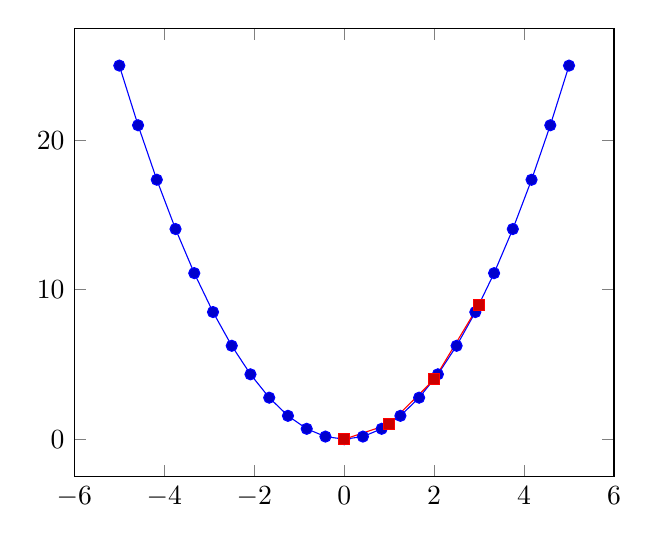
\begin{tikzpicture}
  \begin{axis}
    \addplot {x^2};\addplot coordinates {(0,0) (1,1) (2,4) (3,9)};
  \end{axis}
\end{tikzpicture}

\end{document}
